\chapter{El modelo}
\begin{flushright}
\textit{``Matchmaker, matchmaker,
Make me a match, Find me a find,
Catch me a catch''}
\end{flushright}
\section{Descripción del problema}
Imaginemos que en una ciudad tenemos $m$ universidades y $n$ personas que desean ir a una de estas escuelas, cada universidad tiene un límite alumnos que puede admitir y por esto no todas las personas pueden asistir a su universidad
 ``favorita'', este tipo de cota puede ser común si dos o más escuelas comparten recursos o personal como es el caso de las universidades públicas que dependen en conjunto del presupuesto del gobierno. 
Además, podemos agregar el supuesto de que las escuelas tienen cotas inferiores, usualmente por razones de dinero o de personal a una escuela no le conviene abrir o aceptar a menos de que entren una cantidad considerable de alumnos a está. Adicionalmente, tenemos el supuesto de que todos los alumnos tienen una lista de preferencias no exhaustiva (en muchos casos si es exhaustiva) de qué universidad prefieren y de forma análoga las universidades tienen una lista de preferencias sobre los alumnos, cada escuela y persona tienen necesidades diferentes a los demás, algunos podrían preferir la escuela que está más cerca de sus casas, otros la que te prepara mejor académicamente y otros entre muchas razones podrían preferir la que tenga el mejor ambiente social. 
\\ En notación matemática lo que hacemos es suponer que tenemos $n$ alumnos $\alpha_1, \alpha_2, \ldots, \alpha_n$ y $m$ universidades $a_1, a_2, \ldots, a_m$, con las restricciones: 

\begin{enumerate}
\item \begin{equation} \label{r1}
x_{i,j}= 
\begin{cases}
1 & \qquad \text{si $i$ asiste a la universidad $j$.} \\
0 &\qquad\text{en otro caso.}\ \\ 
\end{cases} \end{equation}
\item \begin{equation} y_{j}= 
\begin{cases}
1 & \qquad \text{si la universidad $j$ abre.} \\
0 &\qquad\text{en otro caso.} \\ 
\end{cases} \end{equation}
\item \begin{equation} \label{r2}
\sum_{j=1}^{m}x_{i,j} \leq1 \ \text{ para toda $i=1,2,\ldots,n$. }
\end{equation} Cada estudiante es admitido en a lo más una universidad. 
\item \begin{equation} \label{r3}
\sum_{i=1}^{n} x_{i,j} \leq M_j\ \text{ para toda $j=1,2,\dots,m$.} 
\end{equation}
Cada universidad tiene un límite de alumnos que puede admitir.
\item \begin{equation} \label{r4}
\sum_{i=1}^{n} x_{i,j} \geq\ m_j\times y_j 
\end{equation}
Cada universidad necesita admitir a una cantidad mínima de alumnos para abrir.
%\item \begin{equation} \label{r5}
%\sum_{i=1}^{n} (x_{i,j}+x_{i,j'}) 
%\begin{cases}
%\geq m_{j,j'} \times y_j \\
%\geq m_{j,j'} \times y_{j'} \\
%\end{cases}
%\end{equation} \\
%para toda $(j,j')$, con $j$ distinto de $j'$. \\
%La cota inferior de las universidades puede ser común.

\item \begin{equation}
\sum_{i=1}^{n} \sum_{j=1}^m w_{j,k} \cdot x_{i,j} \leq N_k\cdot %z_k
\end{equation} 
donde \begin{equation} w_{j,k} \footnote{\text{$w_j,k$ es constante}}= 
\begin{cases}
1 & \qquad \text{si la universidad $j$ es parte de la restricción $k$.} \\
0 &\qquad\text{en otro caso.} \\ 
\end{cases} \end{equation} \\   para toda $k=1,2,\dots,p$   \footnote{Donde $p$ es el número de restricciones comunes.}. \\
La cota superior de las universidades puede ser común.

%\item  \begin{equation} 
%z_{k}= 
%\begin{cases}
%1 & \qquad \text{si las universidades en la restricción $k$ abren.} \\
%0 &\qquad\text{en otro caso.}\ \\ 
%\end{cases} \end{equation}

%\item \begin{equation}
%\sum_{j=1}^{m} w_{j,k} y_{j} \leq z_{k} \text{  para toda $k=1,2,\dots,p$. }
%\end{equation}    \\ Las universidades solo pueden abrir si cumplen su cota común. 

\item \begin{equation} \label{r6}
x_{i,j} \leq y_j \ \text{ para toda $i=1,2,\ldots,n$ y para toda $j=1,2,\ldots,m$.}
\end{equation}
Los solicitantes únicamente pueden asistir a universidades abiertas.

\end{enumerate}

Es importante mencionar que no hay garantía de que todos los alumnos sean admitidos en alguna universidad, algunos se pueden quedar sin estudiar. No todas las universidades necesariamente tienen cotas superiores, inferiores o comunes; en ciertas situaciones se puede considerar que para cierta universidad $j$, $M_{j}$ puede ser igual a infinito o $m_j$ puede ser igual a cero.

Para definir las preferencias de una forma un poco más formal, hacemos uso de la matriz de preferencias

\begin{dfn}
\label{matpref}
Definimos la \textbf{matriz de preferencias} para un problema con $n$ estudiantes y con $m$ universidades como una matriz con $n$ filas y $m$ columnas donde la primera entrada de la celda $(i,j)$ representa el orden de preferencia que le asigna el solicitante $i$ a la universidad $j$ y análogamente la segunda entrada representa el orden de preferencia que le da la universidad $j$ a la persona $i$. La matriz podría tener lugares vacíos en caso de listas no exhaustivas. 
\end{dfn}

Para que dejar más clara la definición es necesario mostrar un ejemplo. 

\begin{eje}
\label{ejemplo matrimonio 1}
Supongamos que contamos con tres solicitantes $\alpha$, $\beta$ y $\gamma$ y con tres universidades $A$, $B$ y $C$ y la matriz de preferencias
$$\begin{pmatrix}
& A & B & C \\
\alpha & 1,3 & 2,2 & 3,1 \\
\beta & 3,1 & 1,3 & 2,2 \\
\gamma & 2,2 & 3,1 & 1,3 
\end{pmatrix}$$
aquí por ejemplo el orden preferencias de $\alpha$ es $(A,B,C)$ y el orden de preferencias de $C$ es $(\alpha, \beta, \gamma)$.
\fin
\end{eje}


Para continuar es necesario introducir un criterio de estabilidad y otro de optimalidad, para ello enunciamos dos definiciones. 

\begin{dfn}{\cite{GaleShapley}}
\label{Estable}
Decimos que una asignación de solicitantes a universidades es inestable si existen dos solicitantes $\alpha$ y $\beta$ asignados a universidades $A$ y $B$ respectivamente, con la propiedad de que $\alpha$ prefiere estar en $B$ que en $A$ y $B$ prefiere tener a $\alpha$ que a $B$. Es decir, existen una universidad y un solicitante que se prefieren entre ellos a sus respectivas asignaciones. 
Además a esto, decimos que una asignación es \textbf{inestable} si existe una universidad cerrada $A$ y $m_j$ solicitantes $\alpha_1,\alpha,2,\dots,\alpha_{m_j}$, con la propiedad de que los $m_j$ solicitantes prefieren estar en $A$ a su situación actual, en este caso se le llama a $A$ \textbf{universidad bloqueadora}.

Alternativamente una asignación de solicitantes a universidades es \textbf{estable} si no es inestable.
\end{dfn}

\begin{dfn}{\cite{GaleShapley}}
\label{optima}
Una asignación es considera \textbf{óptima} si cada solicitante está mejor o igual respecto a sus preferencias que en cualquier otra asignación estable. 
\end{dfn}

A continuación mostramos un par de ejemplos de cómo funcionan las definiciones para dejar todo más claro. 

\begin{eje}
Retomando el ejemplo \ref{ejemplo matrimonio 1}. \\
El conjunto de parejas $(\alpha, A), \; (\beta, B)\; y\; (\gamma, C)$ es estable porque a pesar de las preferencias de las universidades cada persona está con su primera opción, es decir, los solicitantes prefieren a su universidad más que a cualquier otra. Esta además es óptima porque cada solicitante está en su primera opción.
\begin{figure}[H]\centering

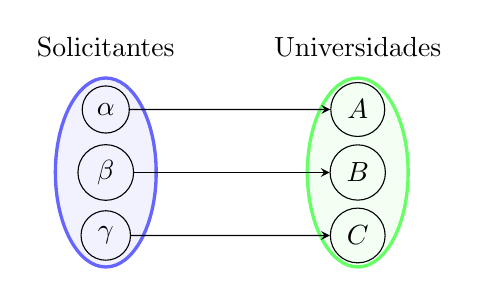
\begin{tikzpicture}[ scale=0.8]
\tikzset{vertex/.style = {shape=circle,draw,minimum size=1.5em}}
\tikzset{edge/.style = {->,> = latex}}
\filldraw[color=blue!60, fill=blue!5, very thick](0,3) ellipse (.8 and 1.5);
\filldraw[color=green!60, fill=green!5, very thick](4,3) ellipse (.8 and 1.5);


% vertices
% 


\node[vertex] (a) at (0,4) {$\alpha$};
\node[vertex] (b) at (0,3) {$\beta$};
\node[vertex] (c) at (0,2) {$\gamma$};


\node[vertex] (e) at (4,4) {$A$};
\node[vertex] (f) at (4,3) {$B$};
\node[vertex] (g) at (4,2) {$C$};


\node (i) at (0,5) {Solicitantes};
\node (j) at (4,5) {Universidades};

\path[-stealth] (a) edge (e);
\path[-stealth] (b) edge (f);
\path[-stealth] (c) edge (g);



%\draw (0.2,8)--(3.8,8);



\end{tikzpicture}

\caption{Emparejamiento estable.}
\end{figure}

\fin
\end{eje}
\begin{eje}
Retomando el ejemplo \ref{ejemplo matrimonio 1}. \\
El conjunto de parejas $(\alpha, A)$, $(\gamma, B)$ y $(\beta, C)$ es inestable porque $\gamma$ prefiere a $A$ que a su universidad actual ($B$) y A prefiere a $\gamma$ que a su universidad actual $(\alpha)$.

\begin{figure}[H]\centering

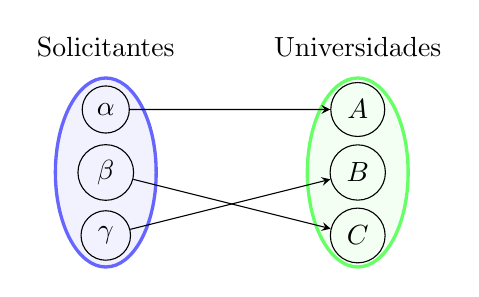
\begin{tikzpicture}[ scale=0.8]
\tikzset{vertex/.style = {shape=circle,draw,minimum size=1.5em}}
\tikzset{edge/.style = {->,> = latex}}
\filldraw[color=blue!60, fill=blue!5, very thick](0,3) ellipse (.8 and 1.5);
\filldraw[color=green!60, fill=green!5, very thick](4,3) ellipse (.8 and 1.5);


% vertices
% 


\node[vertex] (a) at (0,4) {$\alpha$};
\node[vertex] (b) at (0,3) {$\beta$};
\node[vertex] (c) at (0,2) {$\gamma$};


\node[vertex] (e) at (4,4) {$A$};
\node[vertex] (f) at (4,3) {$B$};
\node[vertex] (g) at (4,2) {$C$};


\node (i) at (0,5) {Solicitantes};
\node (j) at (4,5) {Universidades};

\path[-stealth] (a) edge (e);
\path[-stealth] (c) edge (f);
\path[-stealth] (b) edge (g);



%\draw (0.2,8)--(3.8,8);



\end{tikzpicture}

\caption{Emparejamiento inestable.}
\end{figure}
\fin
\end{eje}


Surgen algunas preguntas de aquí ¿siempre existe un emparejamiento estable? ¿cómo se encuentra? Para resolverlas explicaremos un poco sobre algoritmos y su complejidad. Luego, consideraremos el caso en el que $M_j=1$ para toda universidad $j$ y donde además no hay cotas inferiores o comunes, que es mejor conocido como el problema del matrimonio estable. 
